% Copyright 2016 Bas van Meerten and Wouter Franssen
%
%This file is part of ssNake.
%
%ssNake is free software: you can redistribute it and/or modify
%it under the terms of the GNU General Public License as published by
%the Free Software Foundation, either version 3 of the License, or
%(at your option) any later version.
%
%ssNake is distributed in the hope that it will be useful,
%but WITHOUT ANY WARRANTY; without even the implied warranty of
%MERCHANTABILITY or FITNESS FOR A PARTICULAR PURPOSE.  See the
%GNU General Public License for more details.
%
%You should have received a copy of the GNU General Public License
%along with ssNake. If not, see <http://www.gnu.org/licenses/>.

\documentclass[11pt,a4paper]{article}
% Copyright 2016 - 2020 Bas van Meerten and Wouter Franssen
%
%This file is part of ssNake.
%
%ssNake is free software: you can redistribute it and/or modify
%it under the terms of the GNU General Public License as published by
%the Free Software Foundation, either version 3 of the License, or
%(at your option) any later version.
%
%ssNake is distributed in the hope that it will be useful,
%but WITHOUT ANY WARRANTY; without even the implied warranty of
%MERCHANTABILITY or FITNESS FOR A PARTICULAR PURPOSE.  See the
%GNU General Public License for more details.
%
%You should have received a copy of the GNU General Public License
%along with ssNake. If not, see <http://www.gnu.org/licenses/>.


\usepackage[british]{babel}
\usepackage{graphicx,booktabs,listings,amsmath,ifthen,pgfplots,pgfplotstable}
\usepackage[small,bf,nooneline]{caption}
\usepackage{subcaption,longtable}
\usepackage[sort&compress,numbers]{natbib}
\usepackage{tikz,tikz-3dplot}
\usetikzlibrary{backgrounds,arrows,calc}
\usepackage{mathtools}
\usepackage[nottoc]{tocbibind}%adds bibliography to table of contents.
\graphicspath{{./images/}}
%\setlength{\textwidth}{453pt} %597 pt is the a4 paperwidth. Minus 2 in margin. 72 pt = 1 in
%\setlength{\hoffset}{-\oddsidemargin}
%\setlength{\voffset}{-30pt} %
%\setlength{\textheight}{651 pt} %a4 height 845 pt minus 2* total headheight. In this case 2*88pt
%% examine margines via the layout package. Use command \layout{} in document to draw a picture.
%\setlength{\parindent}{0.5 cm}
%\setlength{\parskip}{0 cm}
%\usepackage[left=82pt,right=62pt,top=95pt,bottom=95pt,footnotesep=0.5cm]{geometry}
%\setlength{\headheight}{14pt}

%define colours--------------------
%dark
\usepackage{xcolor}
\definecolor{MyGrayD}{RGB}{1,1,1}
\definecolor{MyRedD}{RGB}{237,45,46}
\definecolor{MyGreenD}{RGB}{0,140,71}
\definecolor{MyBlueD}{RGB}{24,89,169}
\definecolor{MyOrangeD}{RGB}{243,125,34}
\definecolor{MyPurpleD}{RGB}{102,44,145}
\definecolor{MyBrownD}{RGB}{161,29,32}
\definecolor{MyPinkD}{RGB}{179,56,147}
%normal
\definecolor{MyGray}{RGB}{114,114,114}
\definecolor{MyRed}{RGB}{241,89,95}
\definecolor{MyGreen}{RGB}{121,195,106}
\definecolor{MyBlue}{RGB}{89,154,211}
\definecolor{MyOrange}{RGB}{249,166,90}
\definecolor{MyPurple}{RGB}{158,102,171}
\definecolor{MyBrown}{RGB}{205,112,88}
\definecolor{MyPink}{RGB}{215,127,179}
%light
\definecolor{MyGrayL}{RGB}{204,204,204}
\definecolor{MyRedL}{RGB}{242,174,172}
\definecolor{MyGreenL}{RGB}{216,228,170}
\definecolor{MyBlueL}{RGB}{184,210,235}
\definecolor{MyOrangeL}{RGB}{242,209,176}
\definecolor{MyPurpleL}{RGB}{212,178,211}
\definecolor{MyBrownL}{RGB}{221,184,169}
\definecolor{MyPinkL}{RGB}{235,191,217}
%----------------------------------

%Figure ref with hyperref
\newcommand{\fref}[1]{\hyperref[#1]{Figure \ref*{#1}}}
\newcommand{\sref}[1]{\hyperref[#1]{Section \ref*{#1}}}
\newcommand{\tref}[1]{\hyperref[#1]{Table \ref*{#1}}}

%Makes a new command for figures with input values: filename, width(times linewidth),
% caption and label.
\newcommand{\onefigure}[4]{
\setlength{\captionwidth}{#2\linewidth}
\begin{figure}
\includegraphics[width=#2\linewidth]{#1}
\centering
\parbox{\linewidth}{\caption{#3}
\label{#4}}
\end{figure}
}

%Makes a new command for tikz figures with input values: tikz commands, 
% caption and label.
\newcommand{\onetikz}[3]{
\settowidth{\captionwidth}{#1}
\ifthenelse{\lengthtest{\captionwidth<0.7\linewidth}}{\setlength{\captionwidth}{0.7\linewidth}}{}

\begin{figure}
\centering
#1
\centering
\parbox{\linewidth}{\caption{#2}
\label{#3}}
\end{figure}
}

%Makes a new command for two figures next to each other with input values: filename1, caption1, label1,filename2, caption2 and label2. Figure width is set to 0.47\linewidth and the space between the figures is filled with \hfill so the sides of the figures align with to edge of the line.
\newcommand{\twofigure}[6]{
\setlength{\captionwidth}{\linewidth}
\begin{figure*}[ht!]
\begin{minipage}[t]{0.47\linewidth}
\includegraphics[width=\linewidth]{#1}
\centering
\caption{#2}
\label{#3}
\end{minipage}
\hfill
\begin{minipage}[t]{0.47\linewidth}
\centering
\includegraphics[width= \linewidth]{#4}
\centering
\caption{#5}
\label{#6}
\end{minipage}
\end{figure*}
}


%Makes a new command for a table with caption witdh equal to the total table width. Input: tabular, caption and label. Example:
%\onetable{
%\begin{tabular}{ccc}
%a&b&c\\
%\hline
%1&1&1\\
%1&1&1\\
%1&1&1\\
%\end{tabular}
%{The caption.}
%{tab:table1}
%}
\newcommand{\onetable}[3]{
\settowidth{\captionwidth}{#1}
\ifthenelse{\lengthtest{\captionwidth<0.7\linewidth}}{\setlength{\captionwidth}{0.7\linewidth}}{}
\begin{table}
\caption{#2}
\vspace{-0.24cm} %Puts caption close to toprule
\label{#3}
\centering
#1
\end{table}
}

%Makes a long table with captionwidth equal to tablewidth. It takes the following arguments:
%1: Column specifier (e.g. cccc)
%2: Caption
%3: Label
%4: First head (i.e. first row of regular table)
%5: Head of consecutive pages
%6: Foot of pagebreak
%7: Lastfoot (e.g. \midrule)
%8: Body of table
\newcommand{\onelongtable}[8]{
\begin{center}
\settowidth{\captionwidth}{
\begin{tabular}{#1}
#4
#8
\end{tabular}} % This ends the captionwidth part. Next comes the real table.

\begin{longtable}{#1}
\caption{#2}\\
\vspace{-0.74cm} %Puts caption close to toprule
\label{#3}\\

#4
\endfirsthead

#5
\endhead

#6
\endfoot

#7
\endlastfoot

#8
\end{longtable}
\end{center}}




%1:pgfplots code
%2:width
%3:caption
%4:label
\newcommand{\pgfplotsfigure}[4]{
\pgfplotsset{width=#2\linewidth}
\setlength{\captionwidth}{#2\linewidth}
\begin{figure}[t]
\centering
#1
\centering
\parbox{\linewidth}{\caption{#3}
\label{#4}}
\end{figure}
}


\usepackage[bitstream-charter]{mathdesign}
\usepackage[T1]{fontenc}
\usepackage{tcolorbox}
\tcbuselibrary{breakable}
\usepackage[protrusion=true,expansion,tracking=true]{microtype}
\pgfplotsset{compat=1.7,/pgf/number format/1000 sep={}, axis lines*=left,axis line style={gray},every outer x axis line/.append style={-stealth'},every outer y axis line/.append style={-stealth'},tick label style={font=\small},label style={font=\small},legend style={font=\footnotesize}}



%Set section font
\usepackage{sectsty}
\allsectionsfont{\color{black!70}\fontfamily{SourceSansPro-LF}\selectfont}
%--------------------


%Set toc fonts
\usepackage{tocloft}
%\renewcommand\cftchapfont{\fontfamily{SourceSansPro-LF}\bfseries}
\renewcommand\cfttoctitlefont{\color{black!70}\Huge\fontfamily{SourceSansPro-LF}\bfseries}
\renewcommand\cftsecfont{\fontfamily{SourceSansPro-LF}\selectfont}
%\renewcommand\cftchappagefont{\fontfamily{SourceSansPro-LF}\bfseries}
\renewcommand\cftsecpagefont{\fontfamily{SourceSansPro-LF}\selectfont}
\renewcommand\cftsubsecfont{\fontfamily{SourceSansPro-LF}\selectfont}
\renewcommand\cftsubsecpagefont{\fontfamily{SourceSansPro-LF}\selectfont}
%--------------------

%Define header/foot
\usepackage{fancyhdr}
\pagestyle{fancy}
\fancyhead[LE,RO]{\fontfamily{SourceSansPro-LF}\selectfont \thepage}
\fancyhead[LO,RE]{\fontfamily{SourceSansPro-LF}\selectfont \leftmark}
\fancyfoot[C]{}
%--------------------

%remove page number from first chapter page
\makeatletter
\let\ps@plain\ps@empty
\makeatother
%----------------------
\usepackage{color}
\newcommand{\hsp}{\hspace{20pt}}




\usepackage[hidelinks,colorlinks,allcolors=blue, pdftitle={The ssNake tutorial},pdfauthor={W.M.J.\ Franssen}]{hyperref}

\interfootnotelinepenalty=10000 %prevents splitting of footnote over multiple pages
\linespread{1.2}

\usepgfplotslibrary{external}%creates all external tikz images that are included.
\tikzexternalize[shell escape=-enable-write18]%activate externalization
\tikzsetexternalprefix{GeneratedFigures/}
%\tikzset{external/force remake} %Enable forced remake



\begin{document}
%\newgeometry{left=72pt,right=72pt,top=95pt,bottom=95pt,footnotesep=0.5cm}
% Copyright 2016 - 2019 Bas van Meerten and Wouter Franssen
%
%This file is part of ssNake.
%
%ssNake is free software: you can redistribute it and/or modify
%it under the terms of the GNU General Public License as published by
%the Free Software Foundation, either version 3 of the License, or
%(at your option) any later version.
%
%ssNake is distributed in the hope that it will be useful,
%but WITHOUT ANY WARRANTY; without even the implied warranty of
%MERCHANTABILITY or FITNESS FOR A PARTICULAR PURPOSE.  See the
%GNU General Public License for more details.
%
%You should have received a copy of the GNU General Public License
%along with ssNake. If not, see <http://www.gnu.org/licenses/>.

\begin{titlepage}
\begin{center}




% Upper part of the page
{\Huge The ssNake reference manual}
\vfill
\large Wouter Franssen \& Bas van Meerten

\vspace{1cm}
\large Version 1.2b
\vfill

\includegraphics[width=0.5\textwidth]{Images/logo.pdf}\

\vfill
\vfill
% Bottom of the page
{\large \today}

\end{center}

\end{titlepage}


\thispagestyle{empty}
\newpage
\mbox{}

%\restoregeometry

\pagenumbering{roman}
%\pagestyle{empty}
\renewcommand\cfttoctitlefont{\color{black}\Huge\fontfamily{SourceSansPro-LF}\bfseries}
\microtypesetup{protrusion=false} % disables protrusion locally in the document
\tableofcontents % prints Table of Contents
\microtypesetup{protrusion=true} % enables protrusion
\addtocontents{toc}{\protect\thispagestyle{empty}}
%\pagestyle{plain}

\renewcommand\cfttoctitlefont{\color{black!70}\Huge\fontfamily{SourceSansPro-LF}\bfseries}


\pagenumbering{arabic}
\section{Introduction}
ssNake (pronounce `snake') is a versatile tool for processing and analysing NMR spectra, focused on solid-state NMR. The program is both free and open-source and is run from within the python scripting environment, which is also free of charge. ssNake supports a variety of input formats, including Bruker, Varian and Magritek. This tutorial introduces the reader to the ssNake program and its basic controls. The tutorial is aimed at people with a basic understanding of NMR. We refer more experienced users to our reference manual.


\section{Installing ssNake}

The ssNake program consists of a number of python scripts. To be able to run the program you must first install python, and some extra modules for python (mainly Numpy, Scipy and Matplotlib). A short description on how to do this can be found below for several different operating systems.

\subsection{Installing on Windows}
For Windows there are several python distributions around, some of these have all the necessary stuff to run ssNake. Of these, we recommend Anaconda. You can install it in the following way:
\begin{itemize}
\item Go the the Anaconda site (https://www.continuum.io/downloads).
\item Download the Anaconda distribution for Windows (use 32-bit if you do not know what this means)
\item Install Anaconda
\item Reboot your pc or logout/login.
\end{itemize}
Now you have python installed. To install ssNake, copy the ssNake directory to your favourite location (C:\textbackslash{}Program Files\textbackslash{}, for example). ssNake can then be started by double clicking on the `WindowsRun.bat' file. Alternatively, you can execute the `WindowsInstall.vbs' file from within the ssNake directory. This .vbs script creates shortcuts on your desktop and in the startmenu, which you can use to run ssNake. 

\subsection{Installing on Linux}
Installing ssNake on Linux requires installing the required packages. How to do this depends on the Linux distribution you are using. On Ubuntu, you should do the following:
\begin{itemize}
\item Open a terminal
\item Copy the following command : `sudo apt-get install python-matplotlib python-scipy python-numpy'
\item Follow the instructions
\end{itemize}
This should install the packages. ssNake can then be run by navigating to the ssNake directory in a terminal and running `python ssNake.py' from there.


\section{Loading and processing a 1D spectrum}
As a starter, we shall load a 1D spectrum, and start to process this. The data file `1D.json' should be delivered with this document so you can follow all the steps yourself. Firstly, start ssNake by double clicking on the ssNake icon on your desktop (or use another method as described in the installation procedures). This should show something like this (the graphical appearance can be different depending on your operating system):\\
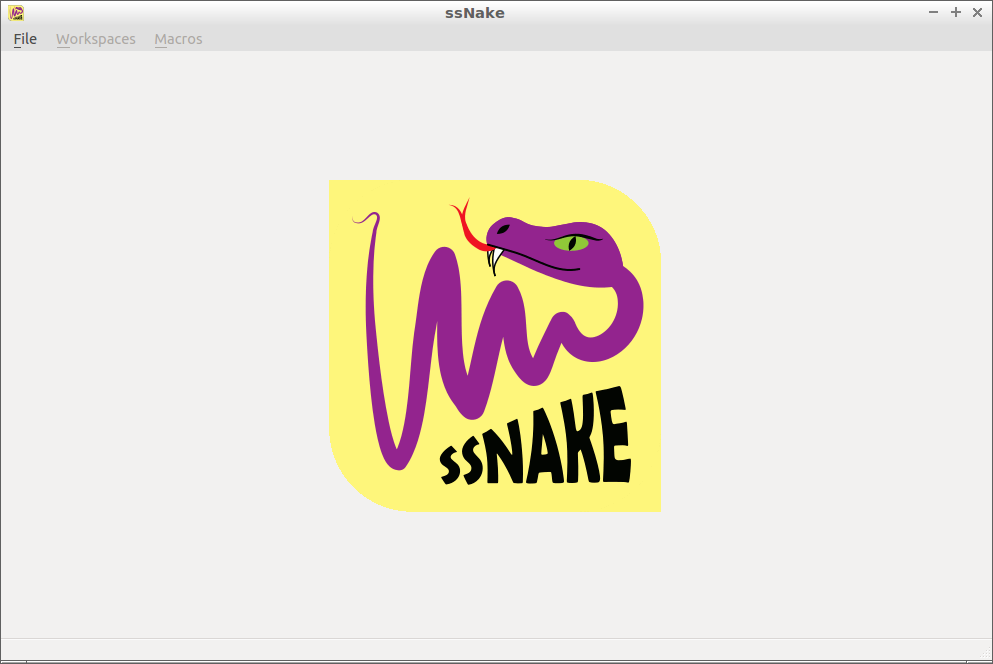
\includegraphics[width=\linewidth]{Images/StartScreen.png}

Now, navigate to the menu on the top of the ssNake screen and choose File $\rightarrow$ Open. This will open a navigation window. Use this window to go to the `1D.json' file that was delivered with this manual and double-click on it to open. ssNake now prompts for a name. This is the name of the data within the ssNake workspace. If you have multiple data files loaded you can switch between them. For now, give it a nice name so you later know which data it is. Say: `1DTest', or something like that. This should give you the following Figure:\\
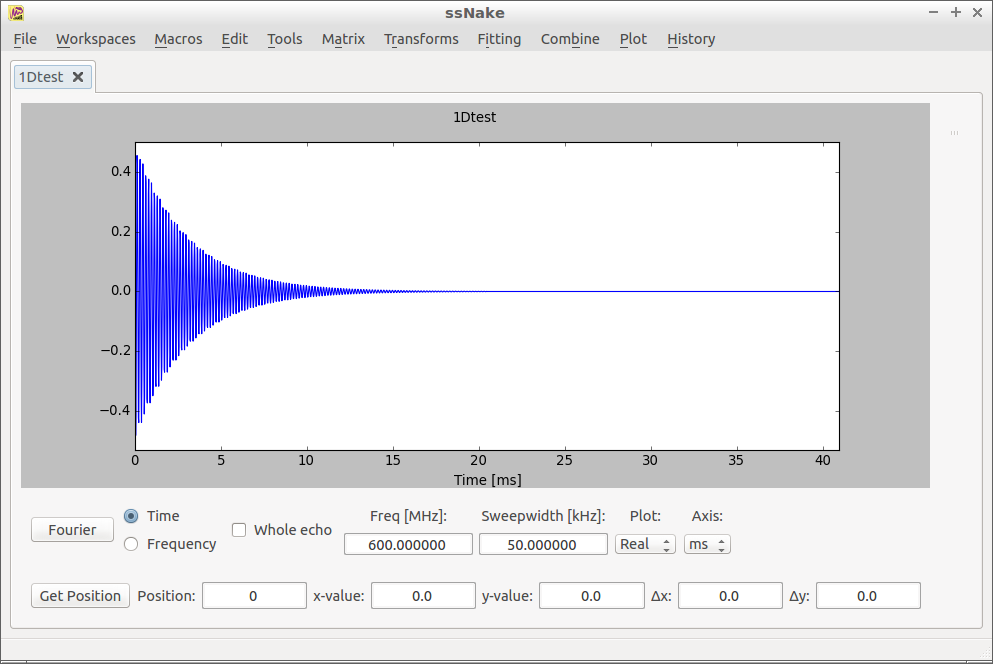
\includegraphics[width=\linewidth]{Images/1Dfid.png}


Now that the data is loaded, we can start processing. As a start, push the `Fourier' button in the lower left corner to perform a Fourier transform. Now we have transformed our time signal to the frequency domain (you can see this by looking at the radio buttons on the lower left of the screen). 
\begin{tcolorbox}[breakable,colback=green!5,colframe=MyBlueD,title=\large Mouse button controls,boxrule=2mm,colback=MyBlueD!30!white]
ssNake provides the user with a nice set of mouse controls to change the view of the graph when the mouse is within the graph area:
\begin{itemize}
\item Clicking and holding the left mouse button, and dragging it creates a zoombox
\item Scrolling with the scroll wheel zooms the y-axis
\item Scrolling with the scroll wheel while holding the right mouse button zooms the x-axis
\item Double clicking the right mouse button resets the view to the full plot limits.
\item Holding the right mouse button and dragging pans the spectrum
\end{itemize}
Play around with these, so you get familiar with them. Some ssNake tools require you to click with the left mouse button on the graph to set some stuff. While using these tools the zoombox function mentioned above is not accessible.
\end{tcolorbox}

The spectrum looks nice, but it is not phased properly. To solve this, go to Tools $\rightarrow$ Phasing. This opens the phasing window. You can now drag the first bar (the `zeroth' order phasing) to the left and right to phase the spectrum. If you are satisfied, push 'apply' to apply the phasing. Remember to click double right to reset the view (all zoom controls can be used during the phasing, except for the zoombox). Most tools in ssNake work in this way: you can view the effects of the tool on the current spectrum or FID, and after you push apply it does the same operation for every trace in the $n$D data. In this case we have 1D data, so `apply' does nothing we haven't already seen on the screen. \\
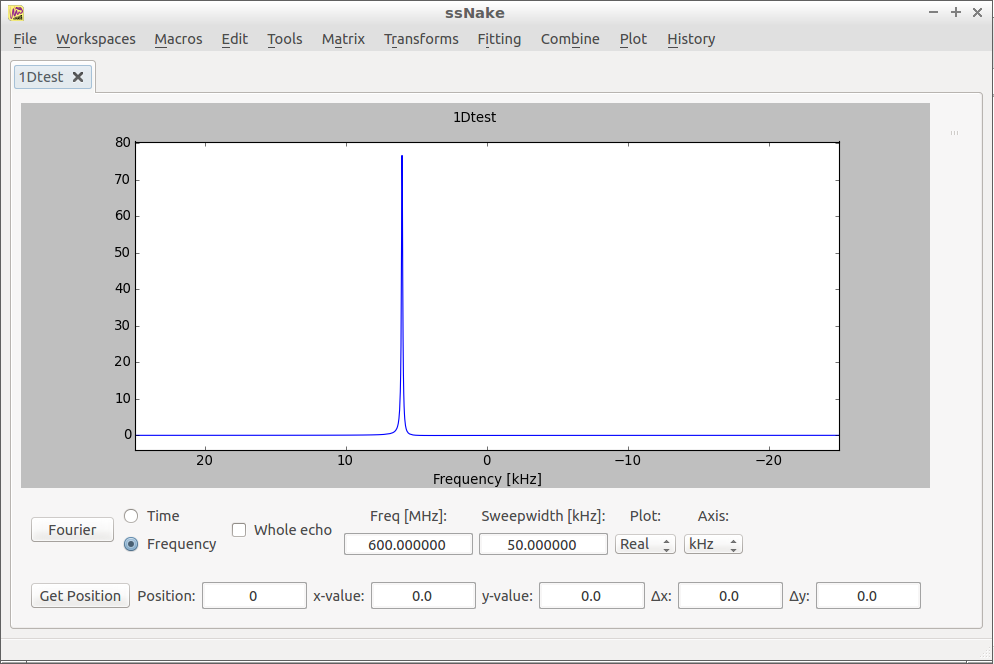
\includegraphics[width=\linewidth]{Images/1DspecPhased.png}

Now that we have processed our first spectrum, it is time to undo it all! ssNake provides an undo and redo button that can undo or redo every action that has been performed on the data. Go to Edit $\rightarrow$ Undo to undo the phasing that we have just applied. Now push ctrl-z to undo the Fourier transform. Equivalently, we can redo this by going to Edit $\rightarrow$ Redo (or by pushing ctrl-shift-z). This shows the unphased spectrum again. To phase it, go to Tools $\rightarrow$ Phasing, but now push `Autophase 0th order' and apply. This asks ssNake to perform the zeroth order phasing himself. Easy, but not always the path to the best phased spectrum! 

\subsection{Noisy data}
Now load another datafile named '1DNoisy.json'. This is the same data as in the previous section, but now with some added noise. Give it a nice name. Fourier transform and phase as you have done before. As you can see, the spectrum is not so nice. To improve this, we can apply some linebroading (or apodization). Go back to the FID, but this time by pushing the `Fourier' button. ssNake knows that you are in a spectrum, so pushing the button now does a reverse Fourier transform. Now go to Tools $\rightarrow$ Apodize and move the slider under `Lorentzian'. While you do this, you can see the FID change. The original signal is altered by a decaying line shown in green. The grey line shows the original data. Choose a nice value and push apply. Now go to the spectrum again via `Fourier' and phase it. This should have improved the spectrum, although you can obscure your signal by applying to much apodization. To see this in a nice way you have to go back to the original FID (without apodization) via the undo controls. Push Fourier to get the noisy spectrum again. Now go to the apodization window, and move the slider again. Apart from apodizing in the time domain, ssNake can also do this in the frequency domain. Now you can see how much you have to apply! This should show something like (I used 200 Hz Lorentzian apodization):\\
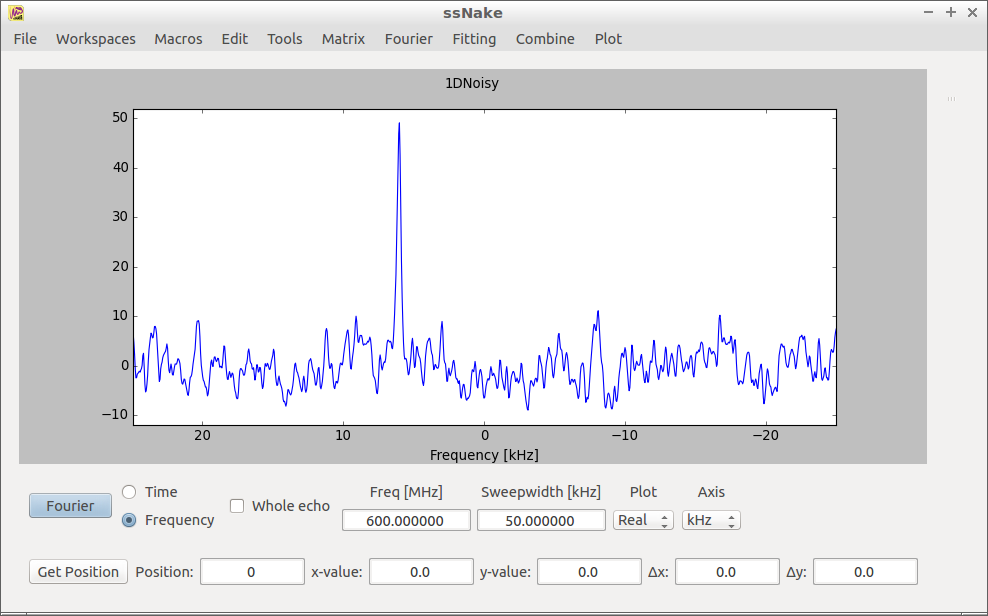
\includegraphics[width=\linewidth]{Images/1DnoisyProcessed.png}

One commonly used value on the `goodness' of a spectrum is the signal-to-noise ratio (SNR). Let's determine this for our noisy spectrum. Go to Fitting $\rightarrow$ S/N. This opens the signal-to-noise window. Now, four values need to be set. The first two are the datapoints were between there is only noise. The second two is the range were our signal is. These can be set by typing into the boxes, but much easier by left-clicking in the spectrum. If you hold your cursor over the spectrum, you will see a vertical dashed line. Moving the mouse moves this line. Now go to the leftmost part of the spectrum and leftclick. This sets the left limit of the noise range. Now move your cursor to the right, but not past the signal and click again. Do the same to select a range which does contain the signal. Push apply to calculate the SNR, which is printed in the box. Cancel closes the window again. Now calculate the SNR for the spectrum with different levels of apodization (remember the option to apodize directly in the spectrum!). More apodization means more signal to noise, unless you overdo it! Also, if you have two resonances close to each other, they will overlap if to much apodization is used.


\begin{tcolorbox}[breakable,colback=green!5,colframe=MyGreenD,title=\large ssNake workspaces,boxrule=2mm,colback=MyGreenD!30!white]
Every time you load new data into ssNake, you are prompted to supply a name. The reason for this is that ssNake supports workspaces, i.e. multiple loaded data files at the same time. You can go to a different workspace (if any) by clicking on itsa respective tab in the top of the ssNake window. Alternatively, use Workspaces $\rightarrow$ Active, and select the name of the desired workspace to go to. Via the same menu you can delete the current workspace, or make a duplicate copy. Some of this can also be done using shortcuts:
\begin{itemize}
\item Next workspace: alt-rightarrow
\item Previous workspace: alt-leftarrow
\item Delete workspace: ctrl-w
\end{itemize}
Note that the workspaces are regarded to form a circle, so pushing alt-rightarrow when you are in the last workspace makes you go back to the first (and vice versa). Changing workspace does nothing to the data and the view of the workspace that you left, so no worries there. Do note, however, that to many open workspaces can take a lot of memory on your computer. Workspaces can also be reorganised by dragging their respective tab to the left or the right.
\end{tcolorbox}

\subsection{Chemical shift referencing}
Until now, we have only viewed the spectrum in it's default settings. For ssNake, this in kHz. However, a commonly used scale in NMR is the parts-per-million scale (ppm). This scale divides the spectrum frequencies by the frequency of the spectrometer, and multiplies by a million. The current noisy spectrum has been measured at a 600 MHz spectrometer. This means that 1 ppm equals 600 Hz (just divide out the million!). To go to a ppm view, ssNake just does this division. Do it by using the dropdown menu under `Axis'.

Now we are in ppm, but the ppm scale is always defined as `x ppm relative to signal y'. The current reference is just the centre of the spectrum (which is now zero), but this is often not correct. Let's just state that the signal we see (which is now at roughly 6.0 ppm) is the true zero point. We must then shift the axis to have `0' at this point. Do it via Plot $\rightarrow$ Reference $\rightarrow$ Set reference. This opens a menu were you can click on the peak in the spectrum (remember to zoom, to be extra accurate). Clicking here sets the frequency (something close to 600 MHz). Leave the zero at `ppm' and the other boxes empty, and push apply. Presto! Now the signal is defined as zero ppm.

Now that we have analysed this data you can close this workspace by going to Workspaces $\rightarrow$ Delete, by typing ctrl-w, or by clicking on the cross button on the tab. Use this to clean up and close all the workspaces. You can view the current workspaces via Workspaces $\rightarrow$ Active. You can click on a non-active workspace to go there, or use alt-rightarrow and alt-leftarrow to cycle through the list.

\section{Fitting a T$_1$ relaxation curve}
ssNake can also be used for fitting exponential decays such as T$_1$ and T$_2$. For this we are going to open a true experimental spectrum measured on one of our Varian spectrometers. Go to Load and navigate to the folder `satrec2D.fid' and open the `fid' file from this folder to load the data. Name it `KI' (it is the $^{127}$I signal of potassium iodide).

You now have loaded a 2D data set. You can see this by looking at the right side of the screen, which now shows a dimension selector with two dimensions. By pushing the radiobutton you can show the signal in another dimension. To view the FIDs measured with different recovery times (as is done in a T$_1$ experiment), click on the \^{} button close to the D1 text. This will cycle through the list of measurements, and will eventually show some signal. Alternatively, it is possible to show them all by going to Plot $\rightarrow$ Stack plot. Push Plot $\rightarrow$ 1D plot, to go back to the original view.

The FID we now see does not have that many points. As the number of points in the FID is equal to the number of points in the spectrum (after we push Fourier), we must increase the number of points to improve the digital resolution of the spectrum. Go to Tool $\rightarrow$ Set size, and fill in `8k' at the `Size' box (ignore the `Offset' box for the time being) and press apply. This will set the number of points to 8192 (one `k' is 1024 points). The new datapoints are zeroes, and are put at the end by default. The signal is now `zerofilled'. The signal is still somewhat noisy, but it is easier to correct this in the frequency domain. Press `Fourier' to go there.

Now we have the spectrum. Due to the nature of the saturation recovery experiment that was performed, the first spectra have hardly any signal. To phase the signal properly, go to the last spectrum via multiple pushes on the up button next to D1. Alternatively, you can go there by typing `$-1$' in the field there and push enter. ssNake uses the regular python definitions for array indexing, meaning that 0 is the first spectrum, and $-1$ is the spectrum before that, which python sees as the last. We can now phase the last spectrum properly (and the phasing will be set for the others too after we push `apply').

Now, we have to apply some linebroading. But let us use a nice trick. Go to Plot $\rightarrow$ Stack plot again. Now open Tools $\rightarrow$ Apodize and move the Lorentzian slider: you can see the effect on all traces! Choose something nice and apply. 

\subsection{The actual fitting}
Now we have `massaged' our data properly, and it is time for the actual T$_1$ fitting. For this we have to make a plot of the intensity of the peak over time. First, get the position of the line
by using the `Get Position' button in the lower left of the screen. Moving the mouse over the spectrum shows a vertical dash. Put your mouse over the highest point of the peak and left-click. Remember that you can still use the scrollwheel (with and without holding the right mouse button) to zoom, to make your pick more precise. The result of our pick will be shown on the bottom line of the screen. `Position' is the value we need, but it also gives the x and y values, and the difference compared to the previous pick in this spectrum.

To get the view we need, we have to type (or copy) this `Position' value to the D2 field, and press `enter'. This will automatically change the view to D1 (see the radio button change), and show the intensity of the peak in time:\\
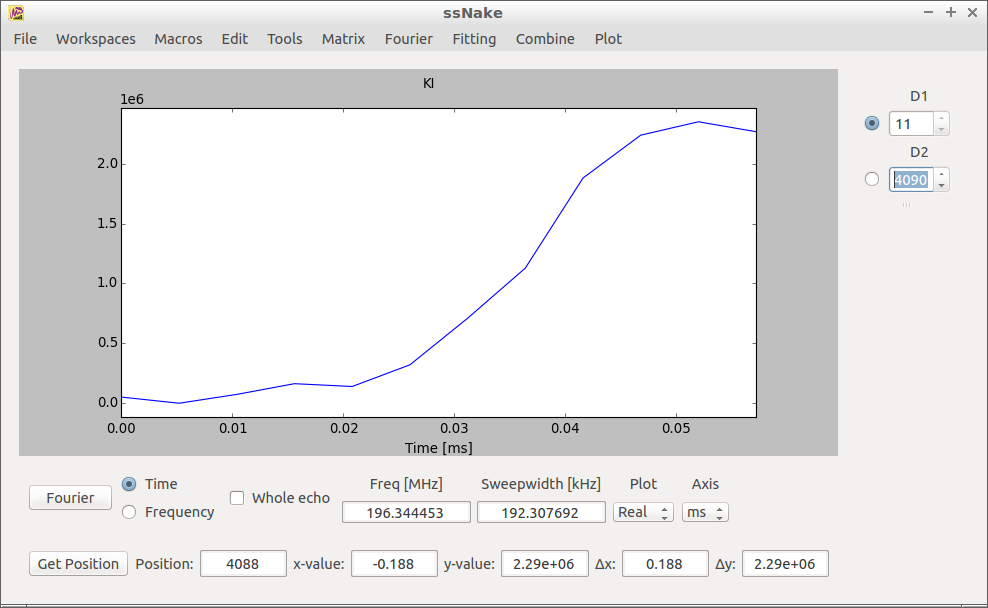
\includegraphics[width=\linewidth]{Images/T1.png}

However, the  current plot is not correct! The data has been measured with an increasing recovery delay, but not a linear one! We must therefore change the current axis to the one we have actually used during the measurement. These spectra have been measured using the `euro' series, as it is effective and easy to remember. If the first delay is, say 1 second, then the euro series of 6 steps is: 1, 2, 5, 10, 20, 50. So the same as the steps in the euro coins. So 1, 2, 5, and then the same times 10, 100, etc. The current spectra have been measured with a euro series starting from 1 ms. First, set the current axis to seconds using the menu in the lower part of the screen. Now we can set the user axis via Plot $\rightarrow$ User x-axis. Here, we must supply a series of numbers equal to the delays we used in the saturation recovery experiment. We have 12 traces (starting with 0.001 s), so the input should be : [0.001,0.002,0.005,0.01,0.02,0.05,0.1,0.2,0.5,1,2,5] . It is quite nasty to type this in every time we do this experiment. ssNake therefore supports the euro series directly. So instead of the mess above, type: euro(0.001) . ssNake knows how many spectra there are, so only the first number in the euro series has to be supplied by the user. Applying should give something like this:\\
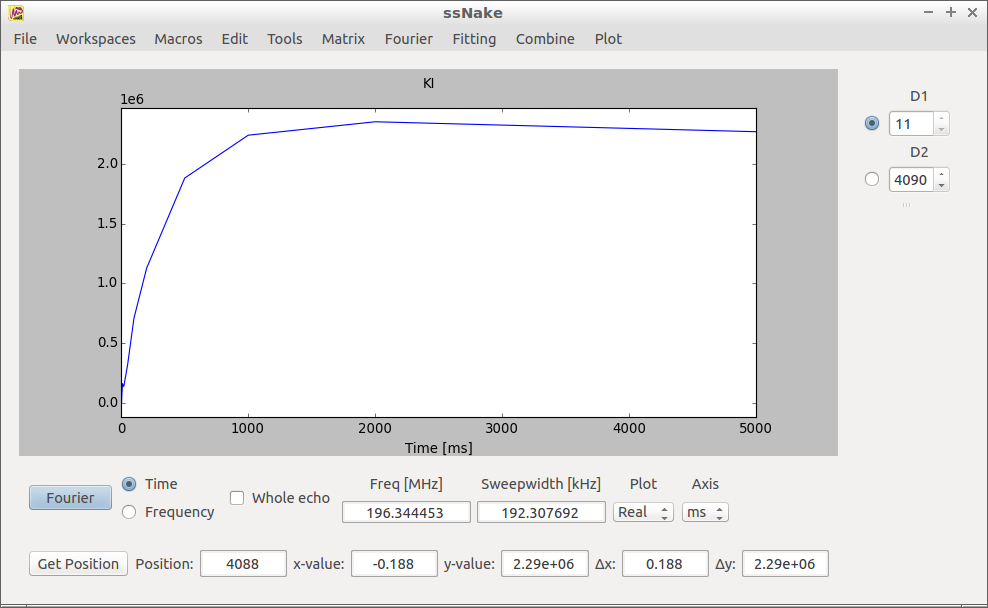
\includegraphics[width=\linewidth]{Images/T1correctAxis.png}


To open the fitting window go to Fitting $\rightarrow$ Relaxation Curve. The current view is now changed to a fitting window. Pushing `fit' performs the fit; `cancel' returns to the regular view. To examine our relaxation curve better it is nice to put the x-axis on log scale (use the checkbox on the screen). Before we perform the fit, we have to set some initial guesses to make sure the fit converges. ssNake puts the amplitude automatically to the value of the last point, so we don't have to worry about this one. For the moment, we can tell ssNake to keep the variable `constant' and `coefficient' static by checking the boxes that are next to them. For the `T' value we have to supply a guess. As the signal is about maximum around 2 seconds, the initial guess of 1 s is quite good, so we keep it there. Now, push `Sim' to show the plot of the current setting. Pretty close already! The fit will certainly converge, so push `Fit'. This should give a value of around 0.3 seconds for this T$_1$. You can now fit it also with `constant' and `coefficient' released. This should give roughly the same T value.

\section{Integrating}
If an NMR experiment is performed in a suitable way, the resulting spectrum is quantitative. That is to say, the number of nuclei that have NMR frequency $a$ are directly proportional to the signal integral of peak $a$. This is used often in NMR to judge the ratio of nuclei between different signals in a spectrum. Naturally, ssNake also supports the calculation of integrals. To start, open `1Dintegrate.json'. As you can see, this is already a spectrum (and it says `Frequency' at the lower left radio buttons). We see two signals, at +10 and -10 ppm. Clearly, they do not have the same height, but how about the integral? Go to Fitting $\rightarrow$ Integrals. This opens a windows were you can select multiple regions for integral calculation. Use the mouse to left-click on the left of the leftmost peak, and then on the right side. Make sure that the whole peak is in the selected region to get a correct integral. The lower boxes now show the selected region and the calculate integral:
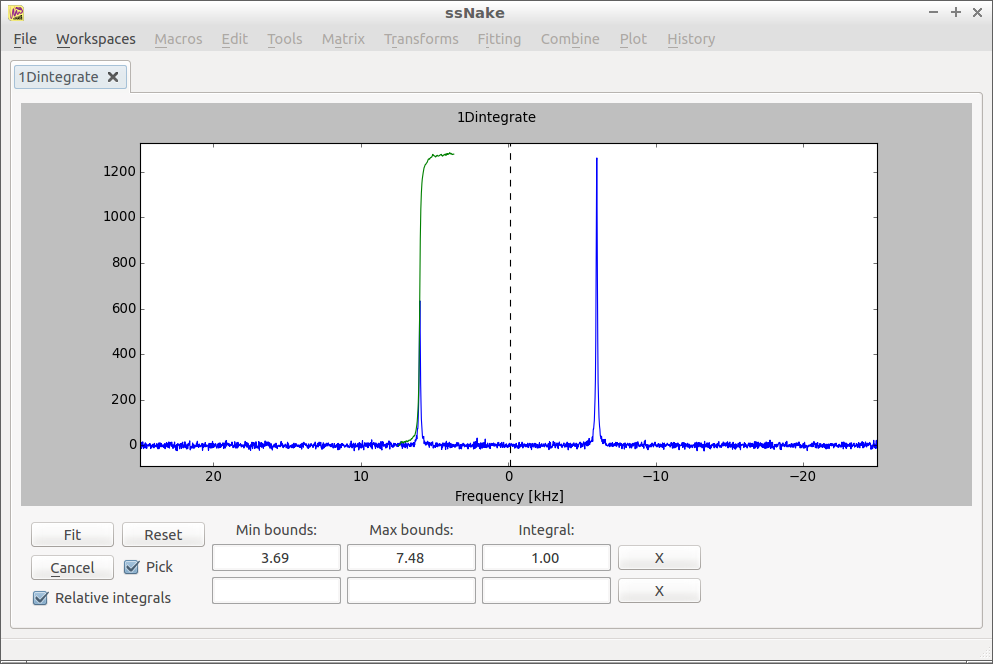
\includegraphics[width=\linewidth]{Images/1Dintegrate.png}


 By default ssNake displays the relative integral: the first integral is set to `1'. You can untick the box `Relative integrals' to show the real integral. Now, select the region of the rightmost peak and put the integrals back to relative. Clearly, the ratio between the peak integrals is about 1:2 (actually, it is exactly two, but the noise limits our accuracy). Now, delete the integral number for the second peak and type `1' in the box and press `enter'. ssNake now scales all the integrals in such a way that this value becomes 1. Pretty neat! Do note that this technique can only be accurately used if the signals do not overlap!



\section{Saving data}
Just as ssNake can load data, it can also save it back to the disk. ssNake currently supports three formats: JSON, .mat and SIMPSON. Of these, the first two save all the relevant data, the SIMPSON format does not include some stuff that ssNake needs to set all parameters right when loading the data again. It is therefore recommended to save the data in one of the two remaining formats. JSON (JavaScript Object Notation) is a plain text format (i.e. you can open it in a regular text editor and view/change the data), while .mat is a binary format. We favour JSON as it is a nice and intuitive format. However, the .mat file is more space efficient, which is useful for larger datasets. Also, as the .mat file is the native format of {\sc Matlab}, it can be loaded in {\sc Matlab} if some extra data manipulation is necessary. You can find the save options in File $\rightarrow$ Save. 

\section{Saving figures}
Apart from saving the raw data, the current figure can also be saved. Open it via File $\rightarrow$ Export $\rightarrow$ Figure. In this windows you can set the title, and the axis labels. Also, the limits of the plot can be set. ssNake supports several formats for saving the figure: SVG, EPS, PDF, PNG and JPEG. If you don't now what this means; just save as PNG. Pushing `Save' opens a file browser to select the name of the new figure.



\section{Final remarks}
This concludes this short `hands-on' tutorial to ssNake. You should now be familiar with the basic controls of ssNake, and be able to process some easy data. More information on ssNake and its controls can be found in the reference manual.







%\bibliographystyle{BibStyle}
%\bibliography{MasterVerslag}

\end{document}
